\documentclass[12pt]{article}
\usepackage{amsmath,amssymb,amsthm}
\usepackage{graphicx,mathabx}
\usepackage{xcolor}
\usepackage{tikz}
\usepackage{cases}
\usepackage{placeins}
\usepackage{lipsum}
\usepackage{mathtools}
\usepackage[shortlabels]{enumitem}
\usepackage{wrapfig}
\DeclarePairedDelimiter{\ceil}{\lceil}{\rceil}
\begin{document}
\title{TCSS 343 - Week 3 - Monday}
\author{Jake McKenzie}
\maketitle
\noindent\centerline{\textbf{Stating Problems Formally and Solving Recurrences}}\\\\\\\\\\\\\\\\
\begin{center}
    ``The object of life is not to be on the side of the majority, but to escape finding oneself in the ranks of the insane". \\$\cdots$\\ Marcus Aurelius
\end{center}
\begin{center}
    ``Treat everyone kindly and light up the night."\\
    $\cdots$\\
    Peter Dinklage
\end{center}
\begin{center}
    ``Computer science got us into this mess. Can computer science get us out of it?"\\
    $\cdots$\\
    Latanya Sweeney re privacy breaches
\end{center}
\newpage
\noindent For this problem consider the problem of finding the product of a list of integers.\\
\centerline{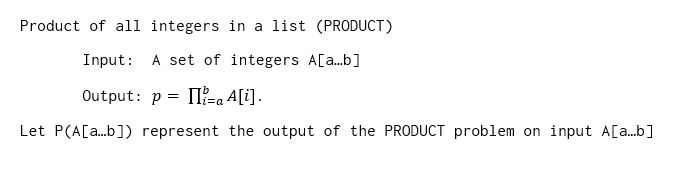
\includegraphics[scale = 0.8]{product.jpg}}
\begin{enumerate}
\item[0. ] State two different self-reductions for the PRODUCT problem. Use the self-reduction 
examples from lecture as a guide. 
\newpage
\item Give recursive algorithms based on your divide and conquer self-reduction to solve 
the PRODUCT problem. 
\item What are the worst case runtimes of the solutions you have generated. (Just state the runtimes. 
You do not need to show your work.)
\newpage
\centerline{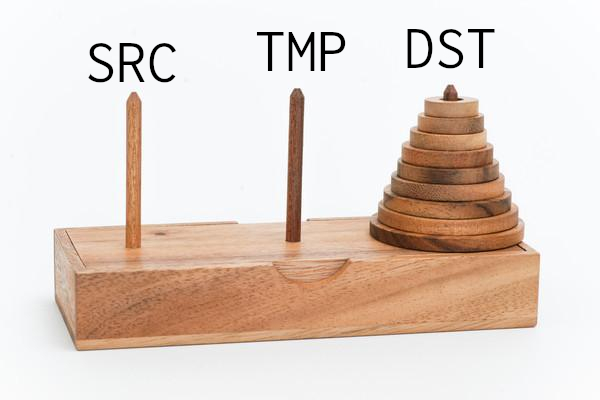
\includegraphics[scale = 1.2]{h0.jpg}}
The \textbf{Tower of Hanoi} has 3 pegs \textit{src}, \textit{tmp} and \textit{dst}. Some disks of different sizes are given which
can slide onto any peg. Initially all of those are in \textit{src} peg in order of size with
largest disk at the bottom and smallest disk at the top. We have to move all the disks
from \textit{src} peg to \textit{dst} peg . At the end, \textit{dst} peg will have disks in the same order of
size. there are some rules :
\begin{enumerate}
    \item[1: ] Only one disk can be moved from one peg to another peg at a time.
    \item[2: ] A disk can be placed only on top of a larger one.
    \item[3: ] A disk can be moved from top only. 
\end{enumerate}
\item  Write a formal statement of this problem. That is, state the input and output criteria as tidy 
as possible.
\newpage
\centerline{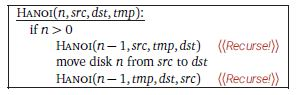
\includegraphics[scale = 0.8]{hanoi.JPG}}
\item Note that the algorithm above does nothing when $n=0$ and only works 
for positive integers in $n$. The recursive algorithm above solves the Tower of Hanoi problem.
Let $T(n)$ denote the number of moves required to transfer $n$ disks(the running time of this algorithm).
The vacuous base case implies that $T(0) = 0$ and I want you to write down the more general recurrence for this problem 
from the algorithm state, then solve for the running time of that algorithm.
\newpage
\item Consider the following recurrence:
\begin{numcases}{T(n)=}
    2, & if $n=1$\\
    3T(\frac{n}{2}) + n, & $n > 1$
  \end{numcases}
Draw out a visualization of what this recurrences looks like as a tree.
\newpage
For the following problems use the recurrence from problem 5 to answer the following problems.
\item How much work is done on level $i$?
\item How many recursive levels are there in the tree?
\item How much work is done at the leaf level?
\item Construct a non-recursive expression equivalent to the recurrence. Your solution may use a summation
\item Use the master theorem to find the big-$\Theta$ bound for the recurrence.
\end{enumerate}
\end{document}










